
\section{Introdução}




\noindent \begin{minipage}[c]{0.6\textwidth}
  \vspace {1cm}
  \begin{description}
    \item [Banana] Exemplo de mini página com figura e seus respectivos rotulos, para que sejam referenciados ao decorrer do texto.
    \item [Maça] Veja que a Figura \ref{fig:place}, está reservando um espaço para adição de figuras, e o mesmo já esta referenciando seu autor e sua nomeclatura com o indice automatico.
  \end{description}

\end{minipage}
\begin{minipage}[c]{0.4\textwidth}
  \captionof{figure}{Placeholder}
  
\includegraphics[width=\textwidth]{figure/placeholder.jpg}
  	\label{fig:place}
    \captionof*{figure}{Fonte: \citeonline{linux:2023}}
\end{minipage}


\section{Desenvolvimento}

\begin{algorithm}[H]
  \SetAlgoLined %APAGAR
  \KwData{Entrada do algoritimo}
  \KwIn{entrada} \
   \KwResult{Resultado do codigo} \
   \While{$x = 0$}{
    Leia atual \;
    \eIf{$n = 2$}{
     vá para aproxima seção \;
     a seção atual se torna esta \;
     }{
     VOlta ao inicio da seção \;
      \Return{EXIT}
    }
   }
   \caption{Nome do algoritimo em Portugues}


\end{algorithm}
\subsection{Método}
\lipsum[2-2]


\subsection{Resultados}
\lipsum[2-2]

\section{Conclusões}

\subsection{Qr CODE}
\par Exemplo de acição de QRcode.
\qrcode {https://dicionario.priberam.org/}
\qquad
QrCode com 5cm:
\quad
\qrcode[height=5cm]{https://github.com/OgliariNatan/Template-UNOPAR}

\subsection{Dicionário}

\par Sugiro este dicionário, para dividas quanto a línga.
\quad
\qrcode {https://dicionario.priberam.org/}

\section{Código externo no main.c}

\lstinputlisting[language=c]{main.c} %Busca os codigos na pasta /cod

\subsection{Banco de dados} \label{Banco de dados}

$\underline{{\color{Blue} }}{\color{red} \, \: \: \left ( \iint_{\widetilde{ \theta }}^{\phi } \right )}  $

\lipsum[2-4]

\subsection{Algoritmo}
\par Um exemplo de adição de Algoritmo. \\

\begin{algorithm}[H]
  \caption{Calculo da potênciação.}
  \label{ap1.2}
  \Entrada{a, b, valor}
  \Saida{Valor da potênciação}
  Var \\
  a, b, valor: inteiro; \Comment {Declara as variável do tipo inteiro.}

  \Inicio{
    escreva ("Você deverá entrar com dois valores, sendo que eles deverão ser
    positivos e inteiros.") \Comment {Inicio do algoritmo.} \\
    escreva ("") \\
    escreva ("Entre com o valor de a:") \\
    leia (a) \\
    escreva("Entre com o valor de b:") \\
    leia(b) \\
    $valor \leftarrow 1$ \\
    \While{$b \neq 0$}{
      $valor  \leftarrow  a  \times valor$ \\
      $b \leftarrow b-1$
    }
    escreval ("A Potência é:", valor)
    }
\end{algorithm}

\section{Resultados e discussões}
%%%%%%%%%%%%%%%%%%%%%%%%%%%%%%%%%%%%%%%%%%%%%%%

\par Aqui vai um exemplo de código em \LaTeX2e.

\begin{algorithm} [H]
	\caption{O nome do código}\label{alg:cap}

	\begin{algorithmic} [H]
		\Require $n \geq 0$	\Comment {n será maior ou igual a zero.}
    \Require $x \geq 10$	\Comment {x será maior que 10.}
		\Ensure $y = x^n$   	\Comment {adicionado.}
    \Ensure $x = n $      \Comment{Idiota.}
		\State $y \gets 1$
		\State $X \gets x$
		\State $N \gets n$
%		\While{$N \neq 0$}
%			\If{$N$ is even}
%			 	   \State $X \gets X \times X$
% 			   	\State $N \gets \frac{N}{2}$  \Comment{Aqui Vai o meu comentario}
%			\ElsIf{$N = 0$ }
%   				 \State $y \gets y \times X$
%  			 	 \State $N \gets N - 1$
%				\State $Xold \gets Xnew$
%			\EndIf
%		\EndWhile
	\end{algorithmic}

\end{algorithm}

\section{Sub Figuras}

\begin{figure}[H] %Figuras da aula pratica 1.1
  \center
  \caption{Resultado da atividade prática 1.2}\label{fig:ap1_cod_vigual1}
  \subfigure[ Algoritmo.\label{fig:pri2}]{
\includegraphics[scale=0.4]{figure/placeholder.jpg}}
  \subfigure[Comportamento.\label{fig:seg2}]{
\includegraphics[scale=.4]{figure/placeholder.jpg}}
  \fontfig{\citeonline{oliveira_SO2009}}

\end{figure}

%%%%%%%%%%%%%%%%%%%%%%%%%%%%%%%%%%%%%%%%%%%%%%%%%%%%%%%%%%
\section{Seção que será apagada}

Para referenciar utilize \cite{ninguem2022curioso}. Também pode ser citado integrada ao texto, de acordo com \citeonline{alguem2022nada}.

Para inserir imagens adicione a figura no diretório \textit{/figure}

\begin{figure}[H]
\centering
\caption{Exemplo de uma imagem bem massa aqui}
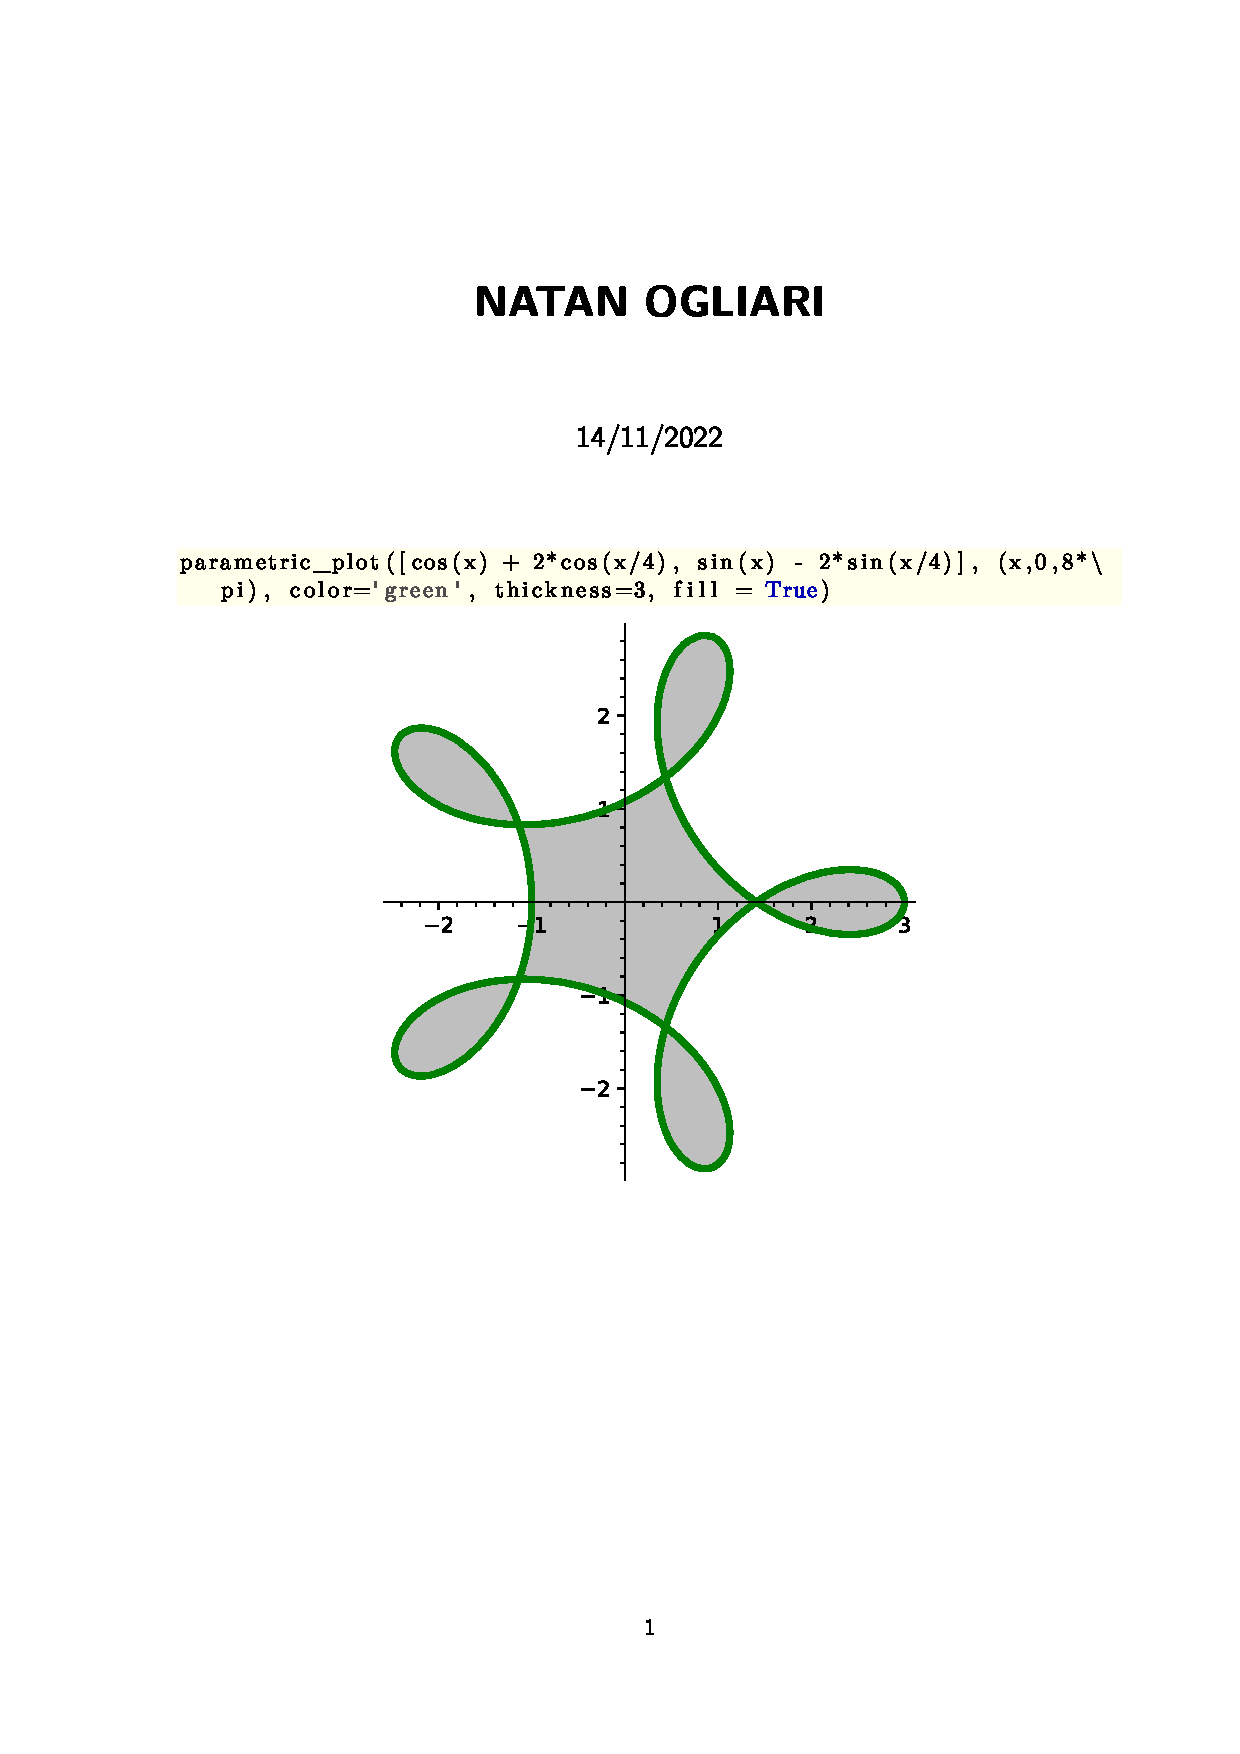
\includegraphics[width=1\textwidth]{figure/Welcome to CoCalc.pdf}
\caption*{Fonte: O autor}
\label{fig:imagem_massa}
\end{figure}

\par Estou usando \href {https://cocalc.com/} {CoCal}

E para referenciar a figura \ref{fig:imagem_massa} utilize dessa forma.

\begin{equation}
  a + b = c \label{1}
  $$ $$ %usado para pular linha
  \sqrt{x} + \sqrt{\smash[b]{y}} + \sqrt{z}
\end{equation}


\par Exemplo de incerção de formula \eqref{1},

\begin{equation}
S = \left\{
\begin{aligned}
  a + b     &= 4\\
  a \cdot b &= 4
\end{aligned}
\right.
$$ $$% Usado para pular linha [não recomendado]
\sum_{n<k,\;\text{$n$ odd}} nE_n
 \label{3}
\end{equation}

Aqui é um exemplo de rodapé. \footnote{Um exemplo de rodapé}

\begin{equation}
\int_{-L}^{L} sen \frac{m \pi x}{2}\,sen \frac{n \pi x}{2}\,dx =
\left \{
\begin{array}{cc}
0, & m \neq n \\
1, & m = n \\
\end{array}
\right.
\end{equation}


\section{Sub itens}

\begin{enumerate}[label=\Roman{*}, ref=(\roman{*})]
  \item fsfsdf
  \item kugfhiuh
\end{enumerate}

\begin{asparaenum}
\item Anterior ... \cite{ninguem2022curioso}
\item Próximo ... \label{pl1}
\end{asparaenum}

\section{Plotação de gráficos}

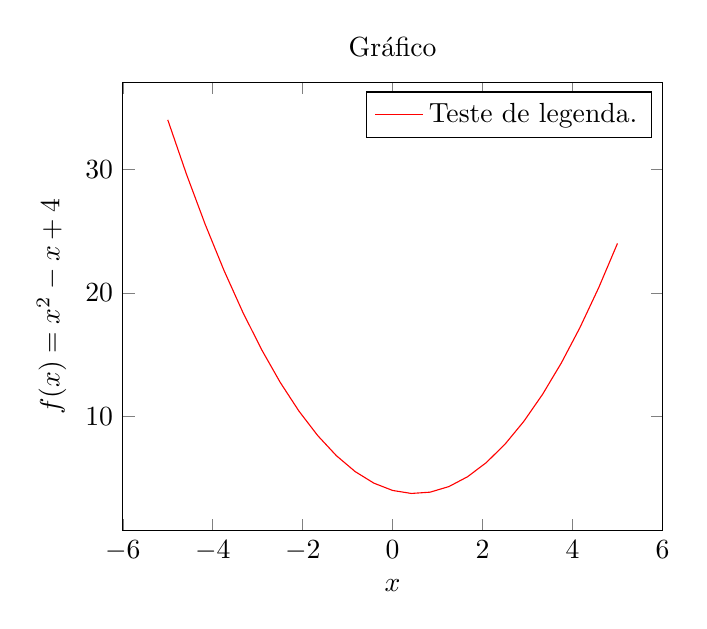
\begin{tikzpicture}

  \begin{axis}[
    title = Gráfico,
    xlabel = $x$,
    ylabel = {$f(x) = x^2 - x +4$}
    ]
    \addplot[color = red] {x^2 - x +4};
    \addlegendentry{Teste de legenda.}

  \end{axis}
\end{tikzpicture}

\subsection{Sub exemplo 3d}
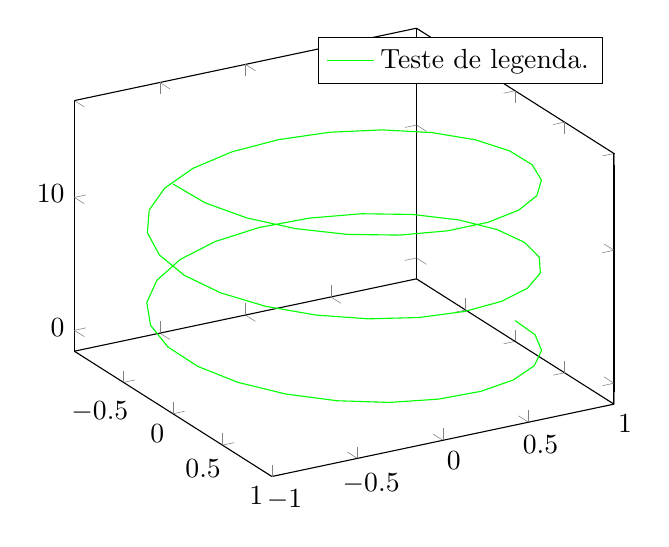
\begin{tikzpicture}
\begin{axis}
    [
    view={60}{30},
    ]
\addplot3[
    title = gráfico 3d,
    domain=0:5*pi,
    samples = 60,
    samples y=0,
]
[color=green]({sin(deg(x))},
{cos(deg(x))},
{x});
\addlegendentry{Teste de legenda.}
\end{axis}
\end{tikzpicture}

\subsection{ Outro exemplo}

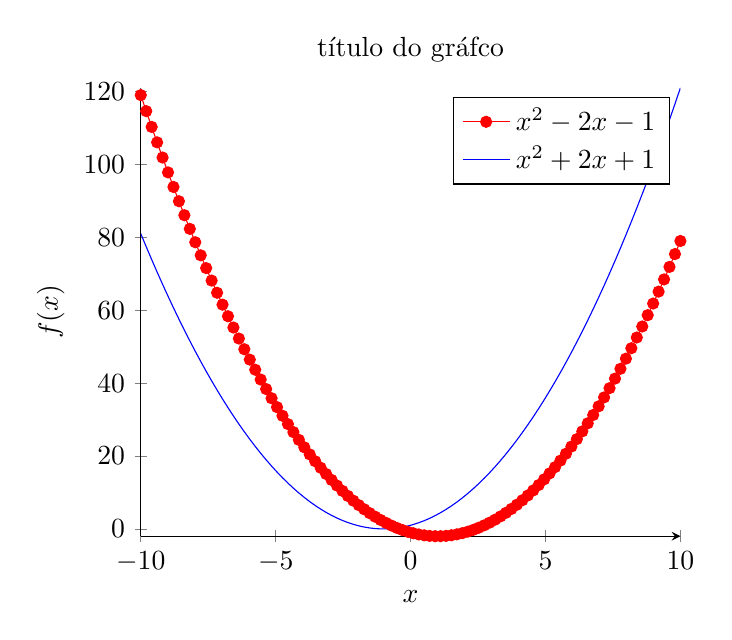
\begin{tikzpicture}
\begin{axis}[
    title = título do gráfco,
    axis lines = left,
    xlabel = \(x\),
    ylabel = {\(f(x)\)},
]
%define a parabula vermelha
\addplot [
    mark=*,
    domain=-10:10,
    samples=100,
    color=red,
]
{x^2 - 2*x - 1};
\addlegendentry{\(x^2 - 2x - 1\)}
%define a parabula azul
\addplot [
    domain=-10:10,
    samples=100,
    color=blue,
    ]
    {x^2 + 2*x + 1};
\addlegendentry{\(x^2 + 2x + 1\)}

\end{axis}
\end{tikzpicture}


\subsubsection{Mais um exemplo}




\begin{figure}
  \caption{Gráfico com arquivo externo}
  \centering
  \begin{tikzpicture}
    \begin{axis}[title = Título do gráfco, xlabel = {$x$}, ylabel = {$y$}, label = grafico]
      \addplot [red] table [x=a, y=c, col sep=comma] {cod/data.csv};
      \addplot [blue] table [x=a, y=b, col sep=comma] {cod/file.csv};
      \addlegendentry{{$x \exp(-x^2-y^2)$}}
    \end{axis}
  \end{tikzpicture}
  \caption*{Fonte: o autor}
\end{figure}



\section{Conclusões}

\begin{algorithm}
\DontPrintSemicolon
\KwData{Ponteiros randomicos.} \Comment{Testando meu comentario} \\
\KwResult{Ordenação de vetores, e concatenação de vetores.}

\Begin{ \Comment{Inicio do meu algoritimo.} \\
$V \longleftarrow X$\;
$S \longleftarrow \emptyset$\;
\For{$x\in X$}{
  $NbSuccInS(x) \longleftarrow 0$\;
  $NbPredInMin(x) \longleftarrow 0$\;
  $NbPredNotInMin(x) \longleftarrow |ImPred(x)|$\;
}
\For{$x \in X$}{
  \If{$ponteiroValido() = 1$ {\bf and} $filaVazia() = 1$}{
    $SOMA4()$}
    }
\nl\While{$S \neq \emptyset$}{\label{InRes1}
\nlset{REM} remove $x$ from the list of $T$ of maximal index\;\label{InResR}
\lnl{InRes2}\While{$|S \cap ImSucc(x)| \neq |S|$}{
\For{$ y \in S-ImSucc(x)$}{
\{ remove from $V$ all the arcs $zy$ : \}\;
\For{$z \in ImPred(y) \cap Min$}{
remove the arc $zy$ from $V$\;
$NbSuccInS(z) \longleftarrow NbSuccInS(z) - 1$\;
move $z$ in $T$ to the list preceding its present list\;
\{i.e. If $z \in T[k]$, move $z$ from $T[k]$ to
$T[k-1]$\}\;
}
$NbPredInMin(y) \longleftarrow 0$\;
$NbPredNotInMin(y) \longleftarrow 0$\;
$S \longleftarrow S - \{y\}$\;
$AppendToMin(y)$\;
}
}
$RemoveFromMin(x)$\;
}
}
\caption{Exemplo de algoritimo}
\end{algorithm}


  %$X \xLongleftarrow[\text{NATAN}]{\text{OGLIARI}} Y $ %COM TEXTO
	% $\uparrow$ %Seta para Cima
	%$\overleftarrow{NATAN}$
